为了清晰、正确地表示视图的轮廓与大小,图纸上所用的线型与尺寸标注,
有统一的标准,现将有关部分简单介绍如下:

\subsubsection{视图中的线型}

\begingroup
\newcommand{\xianxing}[1][]{\tikz \draw[#1] (0,0) -- (3,0);}
\begin{tblr}{hlines,vlines,
    rows={m, rowsep+=3pt}
}
    线型 & 画法 & 主要用途 & 线型粗细标准 \\
    粗实线 & \xianxing[solid, line width=.9mm] & 可见轮廓线 & {粗细为 $b$ \\ $b = 0.1 \text{~} 1.2$ mm} \\
    虚线   & \xianxing[dash pattern=on 15pt off 4pt, line width=.5mm] & 不可见轮廓线 & $\exdfrac{b}{2}$ 左右 \\
    细实线 & \xianxing[solid, line width=.3mm] & 尺寸线、尺寸界线 & $\exdfrac{b}{3}$ 或更细 \\
    点划线 & \xianxing[dash pattern=on 15pt off 3pt on 1pt off 3pt, line width=.3mm] & 轴线和中心线 & $\exdfrac{b}{3}$ 或更细
\end{tblr}
\endgroup

\subsubsection{尺寸注法}

每注一个尺寸时,都要包括下列四个要素:尺寸界线、尺寸线、箭头和尺寸数字,如图 \ref{fig:czjh2-8-23}。

视图上所标注的尺寸是物体的真实大小,与绘图采用的比例尺无关,不标明单位时,是指 mm 。
长度仅用数字表示,
圆的半径在数字前加“$R$”,
圆的直径在数字前加“$\phi$”,
球的直径在数字前加“\mbox{球 $\phi$}”表示。

(1)线段的尺寸注法

尺寸线必须与所注的轮廓线段平行,尺寸界线垂直于被标注的线段。
水平尺寸数字从左到右,铅直尺寸数字从下到上,如图 \ref{fig:czjh2-8-23} 。

\begin{figure}[htbp]
    \centering
    \begin{minipage}[b]{6cm}
        \centering
        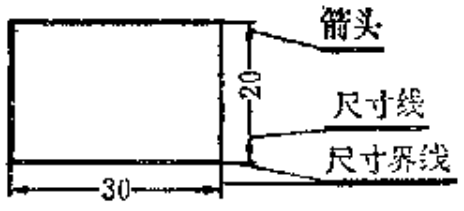
\includegraphics[width=6cm]{../pic/czjh2-ch8-23.png}
        \caption{}\label{fig:czjh2-8-23}
    \end{minipage}
    \qquad
    \begin{minipage}[b]{9cm}
        \centering
        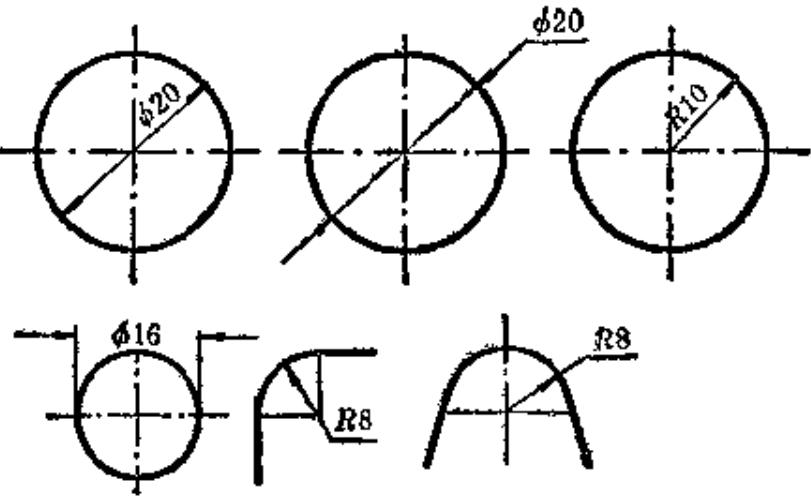
\includegraphics[width=9cm]{../pic/czjh2-ch8-24.png}
        \caption{}\label{fig:czjh2-8-24}
    \end{minipage}
\end{figure}

(2)圆与圆弧的尺寸注法

几种注法如图 \ref{fig:czjh2-8-24} 所示。

